\chapter{The Core Execution Environment}
\label{cee-chapter}

This chapter describes the core execution environment (CEE) of an
SCJVM, which handles execution of an SCJ program.
% The CEE is aware of the structure of Java objects and classes in order
% to handle bytecode instructions properly.
In addition, the CEE of an SCJVM manages the flow of execution
dictated by the SCJ programming model, including, for example,
\texttt{Safelet} setup and mission execution.

This is the part of our SCJVM model that is handled by our compilation
strategy. 
So, it may take the form of a bytecode interpreter, which is the
starting point for the compilation, or C code, which is the output of
the compilation.
We describe both of these in this chapter
(Sections~\ref{cee-launcher-section}, \ref{cee-interpreter-section}
and~\ref{cee-c-code-section}) while the compilation strategy for
transforming between them is described in the next chapter.
We begin with an overview of the CEE's structure in the next section.
We conclude with some final considerations in
Section~\ref{cee-final-considerations-section}.

\section{Overview}

The CEE has three components, two of which depend on whether it is
interpreting bytecodes or executing C code. 
For the CEEs that use a bytecode interpreter, the components are
listed below and shown in Figure~\ref{cee-fig}:
\begin{itemize}
\item the object manager, which manages information about objects
  created during execution of the bytecode;
\item the interpreter itself, which handles execution of bytecode
  instructions; and
\item the launcher, which coordinates the startup of the SCJVM, the
  execution of missions, and the execution of methods in the
  interpreter.
\end{itemize}
% The interpreter is central to the main functionality of the core
% execution environment, but proper handling of infrastructure methods
% requires handling the SCJ mission-based programming model, which is
% dealt with by the launcher.
% The interpreter requires access to memory, but the class information
% and bytecode instructions do not change throughout the execution of
% the SCJVM, so they are provided as global constants in our model that
% are passed to the interpreter as parameters.
% Objects do change throughout the execution of the SCJVM and are in a
% separate region of memory to classes and bytecode instructions.
% The management of objects is handled by the object manager component
% of the core execution environment.

\begin{figure}[bth]
  \centering
  \begin{tikzpicture}

    \coordinate (width)  at (10cm,0cm);
    \coordinate (height) at (0cm,6cm);

    \path (0,0) -- (height)
    coordinate[pos=0.18] (OS boundary)
    coordinate[pos=0.20] (VM part bottom)
    coordinate[pos=0.57] (VM part top)
    coordinate[pos=0.60] (API boundary)
    coordinate[pos=0.82] (App boundary);
    
    \path (VM part bottom) -- (VM part top)
    coordinate[pos=0.7] (CEE part top);

    \path (VM part bottom) -- (VM part top)
    coordinate[pos=0.85] (CEE ypos);

    \path (0,0) -- (width)
    coordinate[pos=0.04] (CEE left)
    coordinate[pos=0.76] (CEE right)
    coordinate[pos=0.78] (VM Services left)
    coordinate[pos=0.96] (VM Services right)
    coordinate[pos=0.01] (CEE part sep);

    \path (CEE left) -- (CEE right)
    coordinate[pos=0.5] (CEE xpos);

    \path (0,0) to node[pos=0.5] (mid) {} (width);
    \path (0,0) to node[pos=0.25] (quart) {} (width);

    \draw (0,0) rectangle (width |- height);

    \draw (OS boundary) -- ++(width);
    \path (0,0) rectangle node[pos=0.5] (OS) {} (width |- OS boundary);
    \draw (mid |- API boundary) rectangle node[pos=0.5] (API) {} (width |- App boundary);
    \draw (App boundary) -- ++(width);
    \path (App boundary) rectangle node[pos=0.5] (App) {} (width |- height);

    \path (quart |- API boundary) rectangle node[pos=0.4] (SCJVM) {} (quart |- App boundary);
    \draw (CEE left |- VM part bottom) rectangle (CEE right |- VM part top);
    \draw (VM Services left |- VM part bottom) rectangle node[pos=0.5] (VM Services) {} (VM Services right |- VM part top);
    \coordinate (CEE) at (CEE xpos |- CEE ypos);

    \node[align=center] at (App)   {SCJ Application};
    \node[align=center] at (API)   {SCJ\\Infrastructure\\and API};
    \node[align=center] at (SCJVM) {SCJ\\Virtual Machine};
    \node[align=center] at (CEE)   {Core Execution Environment};
    \node[align=center] at (VM Services)  {SCJVM\\Services};
    \node[align=center] at (OS)    {Operating System/Hardware Abstraction Layer};

    \foreach \x in {1,...,3}
    \pgfmathsetmacro{\a}{0.33*(\x - 1)}
    \pgfmathsetmacro{\b}{0.33*\x}
    \path ($(CEE left) + (VM part bottom)!0.07!(VM part top)$) -- 
    node[pos=\a] (CEE part \x start) {}
    node[pos=\b] (CEE part \x end) {}
    ($(CEE right) + (VM part bottom)!0.07!(VM part top) - (CEE part sep)$);

    \foreach \x in {1,...,3} 
    \draw ($(CEE part \x start) + (CEE part sep)$)
    rectangle node[pos=0.5] (CEE part \x) {}
    (CEE part \x end |- CEE part top);
    
    \node[align=center] at (CEE part 1) {\small Object \\ \small Manager};
    \node[align=center] at (CEE part 2) {\small Interpreter};
    \node[align=center] at (CEE part 3) {\small Launcher};
  \end{tikzpicture}
  \caption{Structure of an SCJVM, showing the components of the CEE,
    and its relation to the SCJ infrastructure and the operating
    system/hardware abstraction layer}
  \label{cee-fig}
\end{figure}

The components after compilation to C are similar, but the object
manager is replaced with a struct manager, which manages C struct
types representing objects, and the interpreter is replaced with the C
program itself.
The launcher remains unchanged throughout the compilation.
It is assumed that it is already in the form of native code that can
be called from the C code.

The CEE is combined with the SCJVM services to form the complete
SCJVM; this is indicated in Figure~\ref{cee-fig}, which shows the same
structure described in Figure~\ref{scjvm-services-fig} in the previous
chapter, but has a focus on the CEE components.
The SCJVM services are unaffected by the compilation strategy and can
be implemented as a separate library.

Each of the components of the CEE is represented by a single \Circus{}
process in our model.
These processes interact as shown in Figure~\ref{cee-model-fig}.
The overall pattern of the interaction is unaffected by the
compilation, that is, the model of the compiled code has the same
overall flow of communication, although the components have different
names and different channels are used for communication.

\begin{figure}[ht]
  \centering
  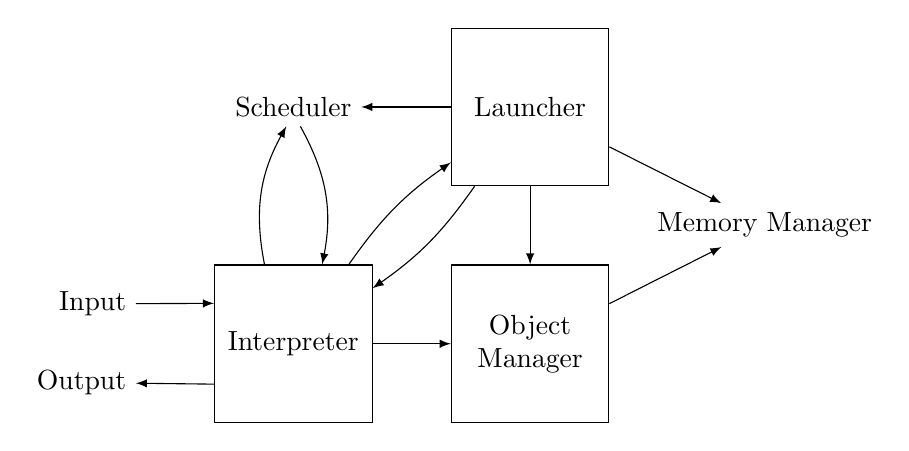
\begin{tikzpicture}
    \node[draw, minimum size=2cm, below right=2cm, align=center]
    (M) {Object\\Manager};
    \node[draw, minimum size=2cm, below=2cm]
    (I) {Interpreter};
    \node[draw, minimum size=2cm, right=2cm]
    (L) {Launcher};

    \draw[-latex, bend left=10] (I) edge (L);
    \draw[-latex, bend left=10] (L) edge (I);
    \draw[-latex] (I) edge (M);
    \draw[-latex] (L) edge (M);
    

    \node[below=1.5cm, right=4.5cm] (MM) {Memory Manager};
    \node[] (S) {Scheduler};
    \draw[-latex] (M) edge (MM);
    \draw (L) edge[-latex] (S);
    \draw (S) edge[-latex, bend left=20] (I);
    \draw (I) edge[-latex, bend left=20] (S);
    \draw (L) edge[-latex] (MM);

    \node[below=2.5cm, left=2cm] (In) {Input};
    \node[below=3.5cm, left=2cm] (Out) {Output};
    \draw[-latex] (In) to (I.153);
    \draw[-latex] (I.207) to (Out);
  \end{tikzpicture}
  \caption{The CEE model processes and their communication with each
    other and the SCJVM services}
  \label{cee-model-fig}
\end{figure}

The launcher manages the startup procedure for the SCJVM and the
execution of missions.
This involves communication with the interpreter (or C program) to
execute initialisation methods.
The interpreter then communicates back with the launcher when it
requires services that are provided by the SCJ infrastructure and API,
such as registering a schedulable object with the current mission.
Allocation of backing stores for the schedulable objects and entering
the corresponding memory areas involves communication with both the
object (or struct) manager in the CEE and the memory manager of the
SCJVM services.
The launcher must also communicate with the scheduler to indicate when
threads should be started or suspended during mission execution.

The interpreter must accept the requests to execute methods on the
main thread from the launcher, and it must also respond to requests
from the scheduler to start the other threads.
When a thread has finished execution, the interpreter signals to the
scheduler that the thread has finished so that it is no longer
scheduled.
The interpreter must also communicate with the launcher to handle
calls to methods that are provided by the SCJ infrastructure, such as
the methods to enter memory areas.
Handling of memory allocation during method execution is performed via
communication with the object manager, which then communicates with
the SCJVM memory manager.
Additionally, the interpreter communicates inputs and outputs to some
console input/output device, which is the only such device required by
the SCJ specification.
Supporting a full range of hardware connections is beyond the scope of
this work.

The interactions just described are modelled by channel
communications.
Those with the SCJVM services memory manager and scheduler use the
channels already described in
Sections~\ref{memory-manager-model-section}
and~\ref{scheduler-model-section}.
The types of values communicated by those channels are also used by
the CEE processes.
These include the type of object identifiers, $ObjectID$, the type of
thread identifiers, $ThreadID$, the type of backing store identifiers,
$BackingStoreID$, and the type of virtual machine data words, $Word$.
We also use the $ClassID$ and $MethodID$ types, which are the types of
class and method identifiers that are declared in the scheduler model
to permit the declaration of the $CEEstartThread$ channel.
Additionally, we declare a field identifier type, $FieldID$.
\begin{zed}
  [FieldID]
\end{zed}
The class, method and field identifiers may be the full names used in
Java class files or some shorter representation, such as unique
identification numbers.
In any case, type information needs to be taken into account so that
methods and fields with the same name, but different type signatures,
have different identifiers.
This is because the identifiers in Java class files include the type
information and the correct operation of method overloading relies on
it.

The channels used for communication between the CEE processes are
summarised in Figure~\ref{cee-channel-table}, with the full channel
declarations shown in Appendix~\ref{cee-model-channels}.
In addition to presenting the name and type for each channel, in the
first two columns of the table.
We also indicate which components of the CEE make use of the channel.
% L - launcher
% I - interpreter
% OM - object manager.
% I/L refers to a channel that is used by both the launcher and
% interpreter, with communications on that channel interleaved.
The channels $output$ and $input$ are used for communication with the
console device mentioned earlier.
As we do not model the console device itself, these are left as
externally visible channels when the component processes are composed
into the complete SCJVM model.
% The fact that they are external channels is indicated by the use of
% \textless{}ext.\textgreater{} in the final columns of the table.
Some channels are marked with various symbols (*, \dag{}, {}+{} and
\ddag{}) so that we can refer to them later in the text.

\begin{table}[t]
  \begin{center}
    \begin{tabular}{@{}lllll}
      \hline
      & Name & Parameter Type & \multicolumn{2}{l}{Communication} \\
      &      &                & from & to     \\
      \hline
      & $executeMethod$ & $ThreadID \cross ClassID \cross MethodID \cross \seq Word$ & L & I  \\
      & $executeMethodRet$ & $ThreadID \cross Word$ & I & L  \\
      & $continueExecution$ & $ThreadID$ & I & L \\
      & $initMainThread$ & $StackID$ & L & I \\ 
      *\dag & $register$ & $ThreadID \cross ObjectID$ & I & L \\
      %* & $registerRet$ & \textless no parameters\textgreater & L & I \\
      *\dag & $enterPrivateMemory$ & $ThreadID \cross \nat \cross ObjectID$ & I & L \\
      *\dag & $executeInAreaOf$ & $ThreadID \cross ObjectID \cross ObjectID$ & I & L \\
      *\dag & $executeInOuterArea$ & $ThreadID \cross ObjectID$ & I & L \\
      \dag & $enterPerReleaseMemory$ & $ThreadID \cross ObjectID$ & I & L \\
      {}+{} & $suspend$ & \textless no parameters\textgreater & I & L \\
      {}+{} & $suspendRet$ & \textless no parameters\textgreater & L & I \\
      {}+{} & $resumeThread$ & $ThreadID$ & I & L \\
      {}+{} & $resumeThreadRet$ & \textless no parameters\textgreater & L & I  \\
      & $output$ & $Word$ & I & \textless ext.\textgreater \\
      & $input$ & $Word$ & \textless{}ext.\textgreater{} & I \\
      & $enterBackingStore$ & $ThreadID \cross BackingStoreID$ & L & OM \\
      & $exitBackingStore$ & $ThreadID$ & L & OM  \\
      & $exitBackingStoreRet$ & $BackingStoreID \cross \boolean$ & L & OM \\
      & $getCurrentAC$ & $ThreadID$ & L & OM \\
      & $getCurrentACRet$ & $BackingStoreID$ & OM & L \\
      & $newObject$ & $ThreadID \cross ClassID$ & I/L & OM  \\
      & $newObjectRet$ & $ObjectID$ & OM & I/L  \\
      \ddag & $getClassIDOf$ & $ObjectID \cross ClassID$ & I/L & OM  \\
      \ddag & $getField$ & $ObjectID \cross FieldID$ & I & OM \\
      \ddag & $getFieldRet$ & $Word$ & OM & I \\
      \ddag & $putField$ & $ObjectID \cross FieldID \cross Word$ & I & OM \\
      \ddag & $getStatic$ & $ClassID \cross FieldID$ & I & OM \\
      \ddag & $getStaticRet$ & $Word$ & OM & I \\
      \ddag & $putStatic$ & $ClassID \cross FieldID \cross Word$ & I & OM \\
      & $addThreadMemory$ & $ThreadID \cross BackingStoreID$ & I & OM \\
      & $removeThreadMemory$ & $ThreadID$ & I & OM \\       
      \hline
    \end{tabular}
  \end{center}
  \caption{The channels used for communication between CEE processes
    before compilation. 
    In the final two columns, L refers to the launcher, I refers to
    the interpreter, OM refers to the object manager, I/L indicates a
    channel shared by the interpreter and launcher in interleaving,
    and \textless{}ext.\textgreater{} indicates and external channel.}
  \label{cee-channel-table}
\end{table}

Most of the channels are part of pairs, with one channel to
communicate a signal to begin an operation and supply any inputs, and
a return channel to communicate back when the operation has finished
and supply any outputs.
The return channel is named by appending $Ret$ to the name of the
channel used to initiate the operation.

There are some channels that deviate this pattern of having a return
channel.
The $executeMethod$ channel is used to signal to the interpreter that
it should begin execution of a method on a given thread.
The interpreter signals on $executeMethodRet$ channel when it has
finished execution of the method.
Since the launcher may need to take some action, such as exiting a
memory area, after the interpreter has finished executing a method,
the interpreter waits until it receives a signal on the
$continueExecution$ channel before continuing to execute.
Since the $continueExecution$ channel forms part of this communication
pattern, it does not have its own return channel.

Before the interpreter can execute methods on the $main$ thread, the
stack space for the $main$ thread must allocated by the launcher and
communicated to the interpreter.
This is handled by the $initMainThread$ channel, which carries the
$StackID$ for the stack space allocated for the $main$ thread.
The interpreter waits for communication on the $executeMethod$ channel
before commencing execution, so the launcher does not need to wait for
the interpreter to finish registering the $main$ thread's stack.

As mentioned above, while executing a method, the interpreter may
signal back to the launcher for handling of special methods.
The channels used for this are the ones marked with a * or a {}+{} in
Table~\ref{cee-channel-table}.
The channels marked with a * represent calls to infrastructure methods
that are part of the SCJ API.
The inputs and outputs of these methods (and hence the types of the
channels associated with them) are taken from the SCJ specification.
The channels marked with a \dag{} are methods that do not return a
value and involve execution of a method in the interpreter as part of
their handling.
Thus, the interpreter waits for a signal on the $executeMethod$
channel after signalling the launcher to handle one of these methods.
The methods marked with a \dag{} do not, therefore, require separate
return channels.
The channels marked with a + expose SCJVM scheduler operations to the
code executed in the interpreter, in order to allow for the
implementation of event handlers. 
Their types follow those of the scheduler's channels.

As mentioned previously, the $output$ and $input$ channels are used to
communicate $Word$ values to and from a console device.
The rest of the channels are used by the launcher and the interpreter
to communicate with the object manager.
The $enterBackingStore$ channel is used by the launcher to signal to
the object manager when a memory area is entered so that it can record
that the corresponding backing store has been entered.
This carries the $ThreadID$ of the thread to be entered, since the
backing stores entered are recorded separately for each thread, and
the $BackingStoreID$ of the backing store to be entered.
There is no corresponding return channel, since it is not necessary
for the launcher to wait while the object manager records the entry to
a backing store.
Similarly, the $exitBackingStore$ channel is used to signal an exit
from the backing store that is the current allocation context of the
given thread.
This does have a return channel, since the launcher must be informed
if the backing store was cleared due to no longer being in use by any
thread.
The $BackingStoreID$ of the exited backing store and a boolean value
indicating if the backing store was cleared are therefore communicated
back to the launcher on a return channel.
Additionally, the $getCurrentAC$ channel (and its return channel) is
used to obtain the $BackingStoreID$ of the backing store used as the
current allocation context for given thread from the object manager,
in order to handle some cases of entering memory areas.

The remaining channels used by the launcher to communicate with the
object manager are used by both the launcher and the interpreter.
These are the $newObject$ channel, which is used to allocate space for
new objects in the current allocation context, and the $getClassIDOf$
channel, which is used to obtain the $ClassID$ for the class of the
object associated with a given $ObjectID$.
% It is used for implementing the \texttt{new} bytecode in the
% interpreter and for creating infrastructure objects in the launcher.
% After compilation it represents a call to a method similar to
% \texttt{malloc()}.
The $newObject$ channel carries the $ThreadID$ of the current thread,
since there is a separate allocation context for each thread, and the
$ClassID$ of the class of the object to be allocated.
The object manager returns the $ObjectID$ of the newly allocated
object via the corresponding return channel.
The $getClassIDOf$ channel carries both the input and output to the
operation on the same channel, since it is a simple data accessing
operation that can be dealt with in a single communication.

The other channels used by the interpreter are the channels for
accessing fields of objects and classes.
The $getField$ channel is used for obtaining the value stored in a
given field of a given object.
It carries the $ObjectID$ of the object whose field is to be accessed
and the $FieldID$ of the field to be accessed.
The object manager then returns the $Word$ value stored in the field.
For putting a value into an object's field, the $putField$ channel is
used, which carries the $Word$ value to store in the field in addition
to the $ObjectID$ and $FieldID$ that identify the object and field to
update.
As this just updates the field and does not return any information,
there is no need for a return channel.
Channels for accessing static fields, $getStatic$ and $putStatic$, are
also provided.
These operate similarly to the channels for object fields but use
$ClassID$ values rather than $ObjectID$ values, since static fields are
attached to classes rather than objects.

The final channels used by the interpreter are the $addThreadMemory$
and $removeThreadMemory$ channels.
The $addThreadMemory$ is used to inform the object manager of a
thread's initial allocation context when the thread starts.
It carries the $ThreadID$ of the thread and the $BackingStoreID$ of
the backing store that serves as the thread's initial allocation
context.
When a thread has finished execution, it informs the object manager
via the $removeThreadMemory$ channel, which carries the $ThreadID$ of
the thread.

As mentioned earlier, some channels used by the interpreter to
communicate with the object manager are replaced with different
channels during compilation.
Those channels are marked with a \ddag{} in
Table~\ref{cee-channel-table}.
After compilation these channels are replaced with channels to obtain
the struct representing the contents of an object and to store an
object’s struct after updating it.
Note that the $getClassIDOf$ channel is shared between the launcher
and interpreter.
After compilation, the interpreter accesses a struct field storing the
$ClassID$ for an object.
However, the launcher is unaffected by the compilation and is agnostic
as to whether the program is in the form of bytecode or C code.
Therefore, the launcher continues to use the $getClassIDOf$ channel
after compilation, which represents a service offered by the object
manager or struct manager to obtain the $ClassID$ by whatever means
are appropriate to the form of the object.
As an optimisation in an implementation, the launcher could be changed
to access struct fields in the same way as the interpreter.
We discuss the form of field accesses in the C code and the channels
used for them in more detail in
Sections~\ref{cee-struct-manager-subsection}
and~\ref{cee-c-program-subsection}.

%\input{../../SCJ-VM/James/LIchans.zed}

%\input{../../SCJ-VM/James/memory_chans.zed}


Next, in Section~\ref{cee-launcher-section}, we describe our model of
the launcher.
We then detail the bytecode interpreter model in
Section~\ref{cee-interpreter-section}, and the C code model in
Section~\ref{cee-c-code-section}.

\section{Launcher}
\label{cee-launcher-section}

As mentioned in the previous section, the launcher is the component of
the CEE that manages the SCJVM startup and coordinates mission
execution.
It is described by the $Launcher$ process.

The launcher remains unaffected throughout the compilation strategy,
because it is agnostic to the class and bytecode information.
However, the launcher must know where to begin execution, so it takes
a parameter, $safeletClass$, which is the $ClassID$ of the
\texttt{Safelet} class.
This can be seen in the the $Launcher$ process definition, the
beginning of which is shown below.

Class initialisers must be executed as part of the SCJVM startup
procedure.
The order in which they are executed is determined by the dependencies
between class initialisers and classes, and is passed to the
$Launcher$ process as a second parameter, $initOrder$, which is a
sequence of $ClassID$s.
\begin{circus}
  \circprocess Launcher \circdef safeletClass : ClassID; initOrder : \seq ClassID \circspot \circbegin
\end{circus}

In what follows, we describe the definition of $Launcher$, focusing on
the aspects relevant for the compilation.
The complete definition can be found in
Appendix~\ref{launcher-appendix}.

The state of the $Launcher$ is divided into three parts.
The first part contains the identifiers of the objects that form the
SCJ mission model, so that the $Launcher$ can call methods of those
objects during SCJVM startup.
The second part contains information on the memory-area objects of
the program, including the relationship between the memory-areas and
the backing stores they represent, so that methods for entering and
exiting memory-areas can be handled.
The final part of the state describes the relationship between the
schedulable objects of SCJ and the threads used by the CEE so that the
threads can be started when mission execution begins.

We use separate Z schemas to specify each part of the state.
The first part is described by the $MissionManager$ schema, shown
below.
It contains the identifiers of three objects:
\begin{itemize}
\item $safelet$, the instance of the class implementing the
  \texttt{Safelet} interface for the program;
\item $missionSequencer$, the mission sequencer
  returned by the safelet's \texttt{getSequencer()} method; and
\item $currentMission$, the mission that is currently executing.
\end{itemize}
Methods of these objects are called at various points throughout SCJVM
startup and mission execution.
\begin{schema}{MissionManager}
  safelet, missionSequencer, currentMission : ObjectID
\end{schema}

The second part of the $Launcher$'s state is described by the
$MemoryAreaManager$ schema below.
It contains the identifiers of the memory-area objects for the
immortal memory, $immortalMemory$, and mission memory,
$missionMemory$.
There is a map, $backingStores$, that relates these identifiers and
the identifiers of the other memory-area objects, to the identifiers
of the backing stores they represent.
We also record the backing store identifiers of the per-release
memories for each thread in the $perReleaseMemories$ map.
Finally, to make sure that nested private memories can be reused,
there is a map from backing store identifiers to the identifiers of
private backing stores they contain, $privateMemoryMap$.
\begin{schema}{MemoryAreaManager}
  immortalMemory, missionMemory : ObjectID \\
  backingStores : ObjectID \finj BackingStoreID \\
  perReleaseMemories : ThreadID \finj BackingStoreID \\
  privateMemoryMap : BackingStoreID \finj BackingStoreID
\where
  \cdots
\end{schema}
Each of the maps in the $MemoryAreaManager$ is injective, since each
memory-area object has a distinct backing store and memory-areas
cannot share a nested private memory-area.
The invariants of $MemoryAreaManager$ are elided above. 
They ensure that each memory-area object has a corresponding backing
store in $backingStores$, and that areas which are not nested private
memories do not appear in the range of $privateMemoryMap$.

The final part of the state is specified in the $SchedulableManager$
schema below.
It contains a map, $schedulableThreads$, from the identifiers of
schedulable objects to the identifiers of the threads associated with
them.
This map must be injective, since every schedulable object has a
separate thread.
\begin{schema}{SchedulableManager}
  schedulableThreads : ObjectID \finj ThreadID
\end{schema}

The state of the process is then the conjunction of these three
schemas.
\begin{circusaction}
  \circstate LauncherState == MissionManager \land MemoryAreaManager \land SchedulableManager
\end{circusaction}

The $Launcher$ state is initialised as described in $LauncherInit$,
which is shown below.
The object identifiers are initialised to the $null$ identifier.
They are later filled with non-$null$ identifiers as the corresponding
objects are created during SCJVM execution.
Similarly, each of the maps is initialised to the empty set.
\begin{schema}{LauncherInit}
	LauncherState~'
\where
	\{ safelet', missionSequencer', currentMission', immortalMemory', missionMemory' \} \\
	\t1 {} \subseteq \{ null \} \\
	backingStores' = \emptyset \\
	perReleaseMemories' = \emptyset \\
	privateMemoryMap' = \emptyset \\
	schedulableThreads' = \emptyset
\end{schema}

The main action of the $Interpreter$ proceeds as shown below.
The state is first initialised as described by $LauncherInit$ and then
the actions $Startup$ and $RunNextMission$ follow in sequence.
$Startup$ defines the SCJVM startup procedure that must be performed
once at the start of SCJVM execution, whereas $RunNextMission$ defines
the procedure that must be performed for each mission run.
We do not handle mission termination in our $Launcher$ model.
This is because the SCJ mission termination procedure has almost no
effect on our compilation strategy; a single mission is sufficient for
our examples to evaluate the compilation strategy.
A formal account of it is available elsewhere~\cite{cavalcanti2013,
  luckcuck2016, zeyda2011}. 
Thus, $RunNextMission$ is only executed once.
\begin{circusaction}
  \circspot \lschexpract LauncherInit \rschexpract \circseq Startup \circseq RunNextMission
\end{circusaction}

The definition of $Startup$ is shown below.
It performs a number of actions in sequence, following the startup procedure for an SCJVM:
\begin{itemize}
\item creating the main thread's stack and passing on the
  $initMainThread$ channel, in $MakeMainStack$;
\item executing the class initialisers in the order given in
  $initOrder$, in $RunClassInitialisers$;
\item creating the immortal memory object that corresponds to the root
  backing store and storing it in $immortalMemory$, in
  $CreateImmortalMemory$;
\item creating the \texttt{Safelet} object and storing it in
  $safelet$, in $CreateSafelet$;
\item calling the \texttt{immortalMemorySize()} and
  \texttt{globalBackingStoreSize()} methods of the $safelet$, and
  checking that the size of the root backing store matches those
  values, in $CheckImmortalMemory$ and $CheckRemainingBackingStore$;
\item calling the \texttt{initializeApplication()} method of the $safelet$, in $InitializeApplication$;
\item calling the $safelet$'s \texttt{getSequencer()} method and
  storing the returned value in $missionSequencer$, in $GetSequencer$;
  and
\item creating the $missionMemory$ object with its corresponding backing store, in $CreateMissionMemory$.
\end{itemize}
\begin{circusaction}
  Startup \circdef MakeMainStack \circseq RunClassInitialisers \circseq CreateImmortalMemory \circseq CreateSafelet \circseq \\
  \t1 CheckImmortalMemory \circseq CheckRemainingBackingStore \circseq InitializeApplication \circseq \\
  \t1 GetSequencer \circseq CreateMissionMemory
\end{circusaction}

$RunNextMission$ begins with calling the \texttt{getNextMission()}
method of $missionSequencer$, in the action $GetNextMission$.
The returned mission is stored in $currentMission$.
Its \texttt{missionMemorySize()} method is then executed, and the
backing store of $missionMemory$ is resized to match, in
$ResizeMissionMemory$.
Next, in $InitializeMission$, the mission's \texttt{initialize()}
method is executed, during which the schedulable objects for the
mission are registered.
Afterwards, in $InitialiseAndStartThreads$, the registered schedulable
objects have their stacks and backing stores created, after which the
threads for all the schedulable objects are started.
Finally, in $WaitForExecution$, the $main$ thread suspends itself and
the $Launcher$ then waits, handling special methods for the threads of
the program when necessary.
Since termination is not handled, this phase of the program continues
indefinitely.
\begin{circusaction}
  RunNextMission \circdef GetNextMission \circseq ResizeMissionMemory \circseq InitializeMission \circseq \\
  \t1 InitialiseAndStartThreads \circseq WaitForExecution
\end{circusaction}

During these actions, methods are executed using the channels
$executeMethod$, $executeMethodRet$ and $continueExecution$, discussed
earlier.
The identifiers of the methods, which may be standard methods from the
SCJ API, or implementation-defined API methods required by the
launcher, are represented by constants in the model.
Although most of the methods used by the $Launcher$ are executed
simply by communicating on each of the channels mentioned above in
turn, as noted above, in $InitializeMission$, the
\texttt{initialize()} method of a mission requires handling of the
\texttt{register()} method for each schedulable object.
We must also provide handling for other special methods.
This is done in the $HandleSpecialMethodsMainLoop$ action below, which
offers handling of the special methods while waiting for return from
the \texttt{initialize()} method on the $executeMethodRet$ channel.
A similar action, without the final choice accepting
$executeMethodRet$, is used to handle special methods in
$WaitForExecution$.
\begin{circusaction}
  HandleSpecialMethodsMainLoop \circdef \circval memoryEntries : ThreadID \fun \nat; \circres retVal : Word \circspot \\
  \t1 (\Extchoice t : ThreadID \circspot \\
  \t2 EnterMemory(t) \circseq \\
  \t2 HandleSpecialMethodsMainLoop(memoryEntries \oplus \{ t \mapsto memoryEntries~t + 1 \}, retVal)) \\
  \t1 {} \extchoice {} \\
  \t1 (\Extchoice t : ThreadID \circspot \\
  \t2 \lcircguard memoryEntries~t > 0 \rcircguard \circguard ExitMemory(t) \circseq \\
  \t2 HandleSpecialMethodsMainLoop(memoryEntries \oplus \{ t \mapsto memoryEntries~t - 1 \}, retVal)) \\
  \t1 {} \extchoice {} \\
  \t1 ((Register \extchoice Suspend \extchoice Resume) \circseq \\
  \t2 HandleSpecialMethodsMainLoop(memoryEntries, retVal)) \\
  \t1 {} \extchoice {} \\
  \t1 (\lcircguard \forall t : ThreadID @ memoryEntries~t = 0 \rcircguard \circguard {} \\
  \t2 executeMethodRet?thr \prefixcolon (thr = main) ?r \then continueExecution!main \then retVal := r)
\end{circusaction}
$HandleSpecialMethodsMainLoop$ takes a value parameter,
$memoryEntries$, which is a map recording how many times a memory area
has been entered for each thread.
It also take a value parameter, $retVal$, which captures the return
value from the execution of the method on the $main$ thread.
It offers a choice of handling a memory-area entry, handling the
corresponding memory-area exit, handling a special method that does
not enter memory-areas, or accepting return from the execution of the
method on the $main$ thread (handled in the usual way using
$executeMethodRet$ and $continueExecution$, with the return value
stored in $retVal$).

$HandleSpecialMethodsMainLoop$ handles memory-area entering
methods, which execute another method after entering a memory-area,
during which further special methods may be called.
Each entry to a memory-area must be matched by a corresponding exit
from the memory-area when this extra method execution returns.
Thus, the entries to memory-areas are tracked in the $memoryEntries$
map.

The number stored in $memoryEntries$ for a thread identifier $t$ is
incremented after handling a memory-area entry on that thread as
described in $EnterMemory(t)$.
Similarly, it is decremented after handling exit from the memory-area
in $ExitMemory(t)$, which is only offered if the value is already
greater than zero.
After handling memory-area entry or exit, or another special method
(handled in the actions $Register$, $Suspend$ and $Resume$),
$HandleSpecialMethodsMainLoop$ recurses to allow further special
methods to be handled.
The return from the top-level method execution on the $main$ thread is
only permitted once all memory areas have been exited and
$memoryEntries$ is zero for all threads.

To illustrate how the nested method execution after memory-area entry
is performed, we show the $ExecuteInAreaOf$ action below, which is one
of the actions offered in external choice in $EnterMemory$, along with
actions to handle other memory-area entering operations.
$ExecuteInAreaOf$ takes a thread identifier $thread$ as a parameter
and only accepts communications from that thread, so that we can
separate out memory-area entries for each thread.
The identifier of a \texttt{Runnable} object, $runnable$, is received
via the $executeInAreaOf$ channel, which is the object that indicates
the method to be executed in the memory-area. 
Such an identifier is received for all of the memory-area entering
methods.
In the case of $ExecuteInAreaOf$, another identifier, $object$, is
also received and a $FindBackingStore$ action is used to communicate
with the memory manager to determine its backing store.
This backing store is then entered, via communication on the
$enterBackingStore$ channel.
The class of the $runnable$ object is determined and its
\texttt{run()} method (represented here by the $run$ identifier) is
executed by signalling on the $executeMethod$ channel.
No communication on the $executeMethodRet$ channel is waited for in
this action, because it is handled separately in the $ExitMemory$
action since other special methods (including further memory entries)
may occur inbetween.
\begin{circusaction}
  ExecuteInAreaOf \circdef \\
  \t1 \circval thread : ThreadID \circspot \circvar runnable, object : ObjectID; bs : BackingStoreID \circspot \\
  \t1 executeInAreaOf?t \prefixcolon (t = thread) ?obj?r \then object, runnable := obj, r \circseq \\
  \t1 FindBackingStore(object, bs) \circseq \\
  \t1 enterBackingStore!thread!bs \then getClassIDOf!runnable?runnableClass \\
  \t1 {} \then executeMethod!thread!runnableClass!run!(\langle runnable \rangle) \then \Skip
\end{circusaction}
The return from the \texttt{run()} method, and the exit from the
memory-area, is specified by the $ExitMemory$ action below.
This, as with the $ExecuteInAreaOf$ action, takes a $thread$
parameter.
A return from a method executing on that thread is accepted on the
$executeMethodRet$ channel, and its return value is discarded as the
\texttt{run()} method is \texttt{void}.
The exit from the memory-area is then performed using the
$exitBackingStore$ and $exitBackingStoreRet$ channels.
The $Launcher$ state may afterwards be updated to account for the
exited memory-area being cleared (due to no longer being in use by any
thread), which is specified in the $ClearPrivateMemory$ schema.
After the exit from the memory-area has been handled, the $Launcher$
signals that normal execution on $thread$ may continue using the
$continueExecution$ channel.
\begin{circusaction}
  ExitMemory \circdef \circval thread : ThreadID \circspot \\
  \t1 executeMethodRet?t \prefixcolon (t = thread) ?void \\
  \t1 {} \then exitBackingStore!thread \then exitBackingStoreRet?bsid?isCleared \then {} \\
  \t1 \circif isCleared = \true \circthen \lschexpract ClearPrivateMemory[bsid/toClear?] \rschexpract \\
  \t1 {} \circelse isCleared = \false \circthen \Skip \\
  \t1 \circfi \circseq continueExecution!thread \then \Skip
\end{circusaction}

The \texttt{register()} method also needs to execute a method in the
interpreter to obtain a thread's priority.
Further special methods are not handled in this case, since the method
to obtain a thread's priority is expected to be a simple method that
does not call special methods.

This handling of special methods is used by the interpreter process
(or C program, after compilation), which must communicate with the
$Launcher$ when such methods are encountered.
To allow for the behaviour of executing methods after entering memory
areas (or during the \texttt{register()} method), the interpreter must
also be prepared to execute another method after signalling to the
$Launcher$.
This is transformed to nested method executions during the compilation
strategy in order to preserve the communication pattern with the
$Launcher$.
We describe in more detail how this communication is performed in the
interpreter in Section~\ref{cee-interpreter-subsection}, and in C
program in Section~\ref{cee-c-program-subsection}.
In the next section, we describe the bytecode interpreter, which,
along with the $Launcher$, forms the CEE before the application of the
compilation strategy.

% \input{../../SCJ-VM/James/launcher.zed}

\section{Bytecode Interpreter Model}
\label{cee-interpreter-section}

This section describes the bytecode interpreter that handles execution
of an SCJ bytecode program.
Its model is composed of two processes:~the model of the object
manager, $ObjMan$, and the model of the interpreter itself,
$Interpreter$.
These are composed together in parallel with the $Launcher$ to form
the complete core execution environment, $CEE$, as shown below.
The synchronisation sets and channel hidings, omitted here, are
consistent with the communication patterns shown in
Table~\ref{cee-channel-table}.
The parameters of each of the components, including the classes, $cs$,
and bytecode instructions, $bc$, which are explained later in this
section, become parameters of $CEE$.
\begin{circus}
  CEE(cs,bc,sid,initOrder) \circdef ObjMan(cs) \parallel
  Interpreter(cs,bc) \parallel Launcher(sid,initOrder)
\end{circus}

In Section~\ref{cee-bytecode-subset-subsection}, we first give an
informal description of the bytecode instructions handled in our model
and the ways in which their SCJ semantics differ from that of standard
Java.
In Section~\ref{cee-classes-subsection}, we describe our model of Java
class information that is used by both $ObjMan$ and $Interpreter$.
The first component, $ObjMan$, is described in
Section~\ref{cee-object-manager-subsection} and the second,
$Interpreter$, in Section~\ref{cee-interpreter-subsection}.

\subsection{Bytecode Subset}
\label{cee-bytecode-subset-subsection}

We model a subset of Java bytecode sufficient to express a wide
variety of SCJ programs and illustrate how further features may be
added, but small enough to permit effective reasoning.
The subset has been chosen by considering the bytecode generated from
a simple SCJ program and removing instructions similar to those
already in the subset.
This ensures the model is not unnecessarily complicated with trivial
or redundant instructions, so we can concentrate on the instructions
that are most of interest in creating the compilation strategy.
The bytecode instructions in our subset are described in
Table~\ref{bytecode-subset-table}.

\begin{table}
  \centering
  \begin{tabular}{llp{8.5cm}}
    \hline
    Instruction & Parameter & Description \\
    \hline
    \texttt{aconst\_null} & (none) & 
    Pushes a null object reference onto the operand stack.
    \\
    \texttt{aload} & local variable index &
    Loads the value from a specified local variable and pushes it
    onto the operand stack.
    \\
    \texttt{areturn} & (none) &
    Returns from the current method, pushing the value on top of the
    current method's operand stack onto the operand stack of the
    method returned to.
    \\
    \texttt{astore} & local variable index &
    Pops a value from the operand stack and stores it in the specified
    local variable.
    \\
    \texttt{dup} & (none) &
    Duplicates the value on top of the operand stack.
    \\
    \texttt{getfield} & constant pool index &
    Pops an object reference from the operand stack, gets the value of
    the field specified by the identifier at the given constant pool
    index for the referenced object, and pushes it onto the operand
    stack.
    \\
    \texttt{getstatic} & constant pool index &
    Gets the value of the static field specified by the field and
    class identifiers at the given constant pool index, and pushes it
    onto the operand stack.
    \\
    \texttt{goto} & program address &
    Unconditionally branches to the given program address.
    \\
    \texttt{iadd} & (none) &
    Pops two integer values from the operand stack, adds them, and
    pushes the result onto the operand stack.
    \\
    \texttt{iconst} & integer value &
    Pushes the given integer value onto the operand stack of the
    current method.
    \\
    \texttt{if\_icmple} & program address &
    Pops two integer values from the operand stack, and branches to
    the given program address if the second value popped is less than
    or equal to the first value.
    \\
    \texttt{ineg} & (none) &
    Pops an integer value from the operand stack, negates it, and
    pushes the negated value onto the operand stack.
    \\
    \texttt{invokespecial} & constant pool index &
    Gets the method and class identifier at the given constant pool
    index and invokes the specified method of the specified class,
    popping the method's arguments, plus a \texttt{this} object
    reference, from the operand stack.
    \\
    \texttt{invokestatic} & constant pool index &
    Gets the method and class identifier at the given constant pool
    index and invokes the specified method of the specified class,
    popping the method's arguments from the operand stack.
    \\
    \texttt{invokevirtual} & constant pool index &
    Gets the method and class identifier at the given constant pool
    index, pops the arguments of the specified method, including a
    \texttt{this} object reference, from the operand stack, and
    invokes the specified method of the class of referenced object.
    \\
    \texttt{new} & constant pool index &
    Allocates a new object of the class specified by the identifier at
    the given constant pool index and pushes a reference to the new
    object onto the operand stack.
    \\
    \texttt{putfield} & constant pool index &
    Pops an object reference and value from the operand stack and
    stores the value in the field specified by the identifier at the
    given constant pool index for the referenced object.
    \\
    \texttt{putstatic} & constant pool index &
    Pops a value from the operand stack and stores the value in the
    static field specified by the field and class identifiers at the
    given constant pool index.
    \\
    \texttt{return} & (none) &
    Returns from a method with no return value.
    \\
    \hline
  \end{tabular}
  \caption{The instructions in our bytecode subset}
  \label{bytecode-subset-table}
\end{table}

Java bytecode instructions operate over a state that records
information on all loaded classes, a stack frame, and the object data
residing in memory.
Various pieces of class information are required for execution of
bytecode instructions, but a constant pool, which stores all the
constants and names required by the class, is the main information
used.

The constant pool contains references to classes, methods and fields
used by the bytecode instructions in the class, as well as constant
values used in the code.
The form of the constant pool is a large array.
Indices into this array are used as parameters to instructions
requiring information from the constant pool.
For example, the \texttt{getfield} and \texttt{putfield} instructions
take constant pool index parameters pointing to a reference to a field
whose value should be obtained or set.
Other class information used at runtime includes information on fields
and methods belonging to the class, which is required for creation of
objects and invocation of methods.

The frame stack forms the second part of the JVM manipulated by
bytecode instructions and consists of a series of frames that contain
the runtime information for each invocation of a method.
When a method is invoked, a new stack frame is created for it and
pushed onto the frame stack, and when the method returns, the stack
frame is popped from the stack.

Each stack frame contains an operand stack, which is used to store
values manipulated by bytecode instructions, and an array of local
variables.
Most bytecode instructions manipulate the operand stack in some way,
popping arguments from it, pushing results to it or performing
specific operations upon it.

The local variables are used to store the arguments of a method and
the results of computations performed on the operand stack.
Operations are not performed directly on the local variables, so the
only bytecode instructions that affect them are those for moving
values between the operand stack and the local variables
(\texttt{aload} and \texttt{astore} are examples of such
instructions).

Some bytecode instructions also manipulate objects, which in our case
reside in backing store memory.
Such instructions include \texttt{new}, which creates objects, and
\texttt{getfield}, which gets the value from a field of an object.
In our choice of instructions for the subset, we mainly focus on
manipulation of objects and method invocation, since those are core
concepts of Java bytecode and require special handling by the
compilation strategy.

The instruction \texttt{dup} is included as an example of a simple
instruction that operates on the operand stack.
It has been chosen for its frequent occurrence in object initialisation.
Other instructions that do simple operand stack manipulation,
including the arithmetic instructions, can be specified similarly.

We also include a few arithmetic instructions as an example of how
integers are handled.
Specifically, we include the integer addition operation,
\texttt{iadd}, as an example of a binary operation, and the integer
negation operation, \texttt{ineg}, as an example of an unary
operation.
We do not include operations for floating point values since the
operations upon them are not substantially different from those on
integers at the level of modelling and compilation.
The model can be easily extended to include more integer operations.

Instructions that create object references (the \texttt{new} and
\texttt{aconst\_null} instructions), pass them around (\texttt{aload},
\texttt{astore}, \texttt{areturn}, etc.), and permit
field accesses (\texttt{getfield} and \texttt{putfield}) are also
included to allow the full range of object manipulations.
We also provide instructions for \texttt{static} field accesses
(\texttt{getstatic} and \texttt{putstatic}) since they are of use in
sharing data between different parts of the program.
However, arrays are not included as they require additional
instructions and can be emulated, albeit inefficiently, with the
instructions given here.

Both the \texttt{invokevirtual} and \texttt{invokespecial}
instructions, which invoke methods on objects, are included.
The \texttt{invokevirtual} instruction looks up the method to invoke
in the method table for the class of the object that the method is
invoked on.
The \texttt{invokespecial} instruction, on the other hand, uses the
class identifier supplied in the method reference pointed to by the
parameter of the instruction when looking up the method.
The \texttt{invokestatic} instruction, for invoking \texttt{static}
methods of classes, is similar to \texttt{invokespecial}, but does not
supply a \texttt{this} object parameter, whereas
\texttt{invokevirtual} and \texttt{invokespecial} pop \texttt{this}
from the stack as an extra argument.

The \texttt{goto} and \texttt{if\_icmple} instructions are provided as
examples of control flow instructions, with \texttt{goto} representing
an unconditional branch and \texttt{if\_icmple} representing a
conditional branch.
Other forms of conditional branch may be implemented in a similar
fashion to \texttt{if\_icmple}, but we do not include those in our
subset since \texttt{if\_icmple} is sufficient to represent most
control flow structures.
Although \texttt{goto} could be represented as a special case of
\texttt{if\_icmple}, we include it as a separate instruction due to
its frequent use in conjunction with \texttt{if\_icmple} to implement
loops.

We do not handle exceptions; errors in the SCJVM are instead handled
by simply aborting execution.
SCJ programs can be statically verified to prove that exceptions will
not be thrown~\cite{kalibera2010,marriott2014}.
Furthermore, reliance on exceptions to handle errors has been
discouraged by an empirical study due to the potential for errors in
exception handling~\cite{sawadpong2012}.
The bytecode instructions that relate to throwing and catching
exceptions are, therefore, not included in our bytecode subset.

As a simplifying assumption, we consider that all values consist of
only a single virtual machine word.
This means that \texttt{long} and \texttt{double} values are not
handled.
Any SCJ API methods that take \texttt{long} or \texttt{double}
arguments are viewed as taking \texttt{int} or \texttt{float} instead.
The reason for this assumption is that handling of two word values
makes little difference at the level of the formal model and our
approach can be easily extended to deal with more types.

Further, we do not make a distinction between the different virtual
machine types in our bytecode instructions.
This is justified as the bytecode instructions simply handle values as
32-bit words, with the type information only used for typechecking
during bytecode validation. 
The code passed into the core execution environment is assumed to have
already passed, which may be done by a separate
component~\cite{klein2003, stark2001, coglio2000, xavier2003}). 
Since many of the instructions behave the same for different types, we
only include those instructions that handle values as object
references.
We would introduce a lot of duplication in the model if, for example,
both the \texttt{areturn} and \texttt{ireturn} instructions were to be
included.

Because we are considering bytecode arising from an SCJ program, some
requirements of SCJ permit further simplifications to our bytecode
subset.
The \texttt{invokedynamic} instruction performs method invocation with
runtime typechecking, mainly for the purpose of implementing
dynamically-typed languages targeting the JVM (though it is also used
to implement the lambda expressions introduced in Java 8).
It is not included in our subset as it does not allow static
typechecking and so should not be used for SCJ.

The requirement for all classes to be loaded at startup greatly
simplifies the semantics of several instructions, since dynamic class
loading does not need to be considered.
It also means that method lookup tables can be precomputed.
This means that the semantics of the \texttt{invokevirtual} and
\texttt{invokeinterface} instructions are the same, since they both
invoke a method on an object, using the object's class as the class
for method lookup.
They, therefore, do not both need to be included and so we have not
included the \texttt{invokeinterface} instruction, since it exists
only to optimise method lookup.

In terms of concurrency considerations, we are assuming our SCJVM to
be single processor, and so we do not need to have more than one
interpreter.
As we see later, the interpreter's threads are modelled using separate
\Circus{} processes, but execution only occurs on one at a time.
We also assume that thread switches can only occur between bytecode
instructions in the interpreter.
This is justified since bytecode instructions should appear to be
atomic.
An implementation may be non-atomic as long as the externally visible
sequence of events is the same as for the model with atomic
instructions.
This means that instructions requiring communication with other
components of the SCJVM, such as \texttt{new}, which communicates with
the memory manager, must be atomic since that they affect shared
state.

Having described our bytecode subset and the assumptions we are
making, we now proceed to describe our model of Java classes in the
next section.

\subsection{Classes}
\label{cee-classes-subsection}

In our model, the information for the Java classes that form the
program is stored in a map, $cs$, that is provided as a parameter to
$CEE$.
The $cs$ map associates $ClassID$s with records of a schema type
$Class$ containing the information for each class.
The $Class$ schema is defined as the conjunction of three schemas,
each defining a different part of the class information.
The first part contains the constant pool and indices into the
constant pool.
The second part contains information on the methods in the class.
The final part contains information on the fields in the class.

The first part is described by the schema $ClassConstantPool$ below.
Its components are $constantPool$, the constant pool itself, and some
indices into $constantPool$:~$this$, referencing the current class,
$super$, referencing the current class' superclass, and $interfaces$,
a set of indices referencing the interfaces implemented by the
current class.
\begin{schema}{ClassConstantPool}
  constantPool : CPIndex \pfun CPEntry \\
  this, super : CPIndex \\
  interfaces : \finset CPIndex
\where
  % the null constant pool entry is not a valid constant pool entry
  nullCPIndex \notin \dom constantPool \\
  % this, super and interfaces must all be valid constant pool indicies (except that super may be null)
  \{this\} \cup (\{ super\} \setminus \{nullCPIndex\}) \cup interfaces \subseteq \dom constantPool \\
  % this, super and interfaces must point to ClassRefs
  constantPool \limg \{this, super\} \cup interfaces \rimg \subseteq \ran ClassRef
\end{schema}
% \begin{schema}{Class}
%   constantPool : CPIndex \pfun CPEntry \\
%   this, super : CPIndex \\
%   interfaces : \finset CPIndex \\
%   methodEntry, methodEnd : MethodID \pfun ProgramAddress \\
%   methodLocals, methodStackSize : MethodID \pfun \nat \\
%   fields, staticFields : \finset FieldID
% \where
%   % the null constant pool entry is not a valid constant pool entry
%   nullCPIndex \notin \dom constantPool \\
%   % this, super and interfaces must all be valid constant pool indicies (except that super may be null)
%   \{this\} \cup (\{ super\} \setminus \{nullCPIndex\}) \cup interfaces \subseteq \dom constantPool \\
%   % this, super and interfaces must point to ClassRefs
%   constantPool \limg \{this, super\} \cup interfaces \rimg \subseteq \ran ClassRef \\
%   \dom methodEntry = \dom methodEnd = \dom methodLocals = \dom methodStackSize \\
%   \forall m : \dom methodEntry @ methodEntry~m \leq methodEnd~m \\
%   % a method's local variables must at least include space for its arguments
%   \forall m : \dom methodLocals @ methodArguments~m \leq methodLocals~m
% \end{schema}
The entries of $constantPool$ are indexed by a type $CPIndex$.
In the JVM, the $CPIndex$ values are positive integers, but no
arithmetic or comparison is performed on constant pool indices in our
model so we do not represent that fact.

We distinguish one particular $CPIndex$ value, a constant
$nullCPIndex$, which represents an invalid index into the
$constantPool$.
It is used as a placeholder in cases when no index is present.
For example, the class \texttt{Object} has no superclass, so the index
of the constant pool entry referencing its superclass is
$nullCPIndex$.

Each of the entries in the $constantPool$ is represented by a free
type $CPEntry$, the definition of which is shown below.
It has three constructors:~$ClassRef$, representing a reference to a
$ClassID$, $MethodRef$, representing a reference to a method of a
particular class by a $ClassID$ and $MethodID$, and $FieldRef$,
representing a reference to a field of a particular class by a
$ClassID$ and $FieldID$.
\begin{zed}
  CPEntry ::= \\
  \t1 ClassRef \ldata ClassID \rdata | MethodRef \ldata
  ClassID \cross MethodID \rdata | FieldRef \ldata ClassID \cross
  FieldID \rdata
\end{zed}
Although there are other types of constant pool entry described in the
JVM specification, we do not include them in our model since some of
them are not relevant to our subset. 
Examples of such entries are those containing information for the
$invokedynamic$ instruction or containing constant values which are
pushed onto the stack by instructions not in our subset.
Some constant pool entries are used by other constant pool entries.
For example, in the JVM specification, method references reference
another constant pool entry, which in turn contains references to
further constant pool entries with string representations of the
method's name and type.
In our model, we hide this complexity in the identifier types
$ClassID$, $MethodID$ and $FieldID$, omitting the extra constant pool
entries.
Thus, the $CPIndex$ values will be in the domain of $constantPool$
will not necessarily be sequential.

The first invariant of $ClassConstantPool$ requires that $nullCPIndex$
not be in the domain of $constantPool$, since $nullCPIndex$ is not a
valid index into $constantPool$.
The second invariant of $ClassConstantPool$ states that the indices
$this$, $super$, and $interfaces$ must be in the domain of
$constantPool$, unless $super$ is $nullCPIndex$ (which will be the
case for the \texttt{Object} class).
Finally, the third invariant requires that the $constantPool$ entries
at $this$, $super$ and $interfaces$ are $ClassRef$s.

The second part of the class information is defined by $ClassMethods$,
shown below.
This is separate from $ClassConstantPool$ since the methods of a class
will not necessarily appear in its constant pool.
Only methods called by the bytecode of a class' methods will appear in
its constant pool.
The components of $ClassMethods$ are maps from $MethodID$ values to
the information about each method.
The first two, $methodEntry$ and $methodEnd$, map to $ProgramAddress$
values, which are indices into a separate bytecode array representing
the start and end points of the method.
The last two components, $methodLocals$ and $methodStackSize$, map to
natural numbers giving the required number of local variables and
operand stack slots for the method.
These values are used during the compilation strategy to declare C
variables to store the local variables and operand stack values.
\begin{schema}{ClassMethods}
  methodEntry, methodEnd : MethodID \pfun ProgramAddress \\
  methodLocals, methodStackSize : MethodID \pfun \nat
\where
  \dom methodEntry = \dom methodEnd = \dom methodLocals = \dom methodStackSize \\
  \forall m : \dom methodEntry @ methodEntry~m \leq methodEnd~m \\
  % a method's local variables must at least include space for its arguments
  \forall m : \dom methodLocals @ methodArguments~m \leq methodLocals~m
\end{schema}
In addition to the components of $ClassMethods$, we declare a global
function $methodArguments$ from $MethodID$s to natural numbers, which
gives the number of arguments that each method takes.
This is a global function since each $MethodID$ encodes the type of
the method, so the number of arguments for a method can always be
determined from its identifier.
The $methodArguments$ function is also total for this reason.
We use $methodArguments$ in one of the invariants of $ClassMethods$,
and also in the $Interpreter$ and compilation strategy when handling
method calls.

The first invariant of $ClassMethods$ requires that all the component
maps have the same domain, so that all the information must be
supplied for any method present in the class.
The second invariant requires that the $methodEntry$ for each method
be before its $methodEnd$.
Finally, the third invariant requires that $methodLocals$ be large
enough for each method to contain its $methodArguments$, since each
argument of a method is stored in a local variable.

The final part of the class information is given in the $ClassFields$
schema below.
It contains two sets of $FieldID$s, $fields$ and $staticFields$, which
are the identifiers of the class' object fields and static fields
respectively.
The static and non-static fields need to be distinguished so that we
know where each needs to be stored:~static variables have only one
copy for each class, whereas non-static fields are stored separately
for each instance of a class.
The $fields$ and $staticFields$ sets are required to be disjoint since
no field can be both static and non-static.
\begin{schema}{ClassFields}
  fields, staticFields : \finset FieldID
\where
  fields \cap staticFields = \emptyset
\end{schema}

The three schemas containing the different parts of the class
information are conjoined together to form $Class$, as shown below.
\begin{zed}
  Class == ClassConstantPool \land ClassMethods \land ClassFields
\end{zed}

In addition to defining $Class$, we also define functions for
extracting information from the $constantPool$ for a given $Class$, in
order to make specifying things about them easier.
Since the functions are just abbreviations of data access operations,
we omit them here.

We also require a way of expressing the fact that one class is a
subclass of another.
For this, we define some relations between classes.
The $\directsubclass$ relation, shown below, defines what it means for
two $Class$ schemas to represent classes in a direct subclass
relationship.
A $Class$, $c1$, is a direct subclass of another $Class$, $c2$, if the
identifier at the $this$ index for $c2$ is the identifier at $super$
for $c1$, or the identifier at one of $c1$'s $interfaces$ indices.
This treats both the case where $c2$ is the superclass of $c1$ and the
case where $c2$ is an interface implemented by $c1$.
The functions $superClassID$, $thisClassID$ and $interfacesClassIDs$
are used in this definition to extract the $ClassID$ values at
$super$, $this$ and $interfaces$ respectively from the $constantPool$.
\begin{axdef}
  \_ \directsubclass \_ : Class \rel Class
  \where
  \forall c1, c2 : Class @ c1 \directsubclass c2 \iff {} \\
  \t1 (c1.super \neq nullCPIndex \land superClassID~c1 = thisClassID~c2) \\
  \t1 {} \lor thisClassID~c2 \in interfacesClassIDs~c1
\end{axdef}
Another relation, $subclassRel$ is defined in terms of
$\directsubclass$ to specify when a $ClassID$ refers to a class that
is a subclass of the class referenced by another $ClassID$.
In order to define this, we require a mapping from $ClassID$ to
$Class$, so $subclassRel$ is defined in terms of a function from such
a mapping to a relation on $ClassID$.
A technical issue prevents $subclassRel$ from being used as an infix
relation due to this.

The definition of $subclassRel$ is shown below.
Given a mapping $cs$ from $ClassID$ to $Class$ that is consistent with
the information at the $this$ entry in the $constantPool$,
$subclassRel~cs$ relates two $ClassID$ if they are in the domain of
$cs$ and their corresponding $Class$es would be related under
$\directsubclass$.
The $subclassRel$ is also taken as a reflexive transitive closure so
that it represents the relationship between a $ClassID$ and any
$ClassID$ it could be used in place of.
\begin{axdef}
  subclassRel : (ClassID \pfun Class) \fun (ClassID \rel ClassID)
  \where
  \forall cs : ClassID \pfun Class | (\forall c : \dom cs @ thisClassID~(cs~c) = c) @\\
  \t1 (\forall c1, c2 : ClassID @ (c1, c2) \in subclassRel~cs \iff (\{c1,c2\} \subseteq \dom cs \land cs~c1 \directsubclass cs~c2)) \\
  \t1 \land subclassRel~cs = (subclassRel~cs)^*
\end{axdef}

The $cs$ map provided as a parameter to $CEE$ is used as the parameter
to $subclassRel$ in each of the processes that uses it.
In order to ensure $CEE$ works correctly (in particular, that it is
divergence-free), several restrictions are placed on $cs$.
One of these is the requirement that $Class$ associated with each
$ClassID$ have its $this$ reference be the same as that $ClassID$,
which is part of the $subclassRel$ definition.
Further restrictions include having all superclasses present in the
map and ensuring the ranges defined by $methodEntry$ and $methodEnd$
for each $Class$ are disjoint.
These restrictions are also used as assumptions in the compilation
strategy laws.
A full formal statement of the restrictions is given in the definition
of a $cs$ constant in Appendix~\ref{constants-appendix}, which is used
to instantiate the $cs$ parameter of $CEE$.
The inputs to the interpreter and compilation strategy are expected to
be refinements of the constant in Appendix~\ref{constants-appendix}.

We next describe the object manager process, $ObjMan$, which uses the
$Class$ type and the $cs$ map.

\subsection{Object Manager}
\label{cee-object-manager-subsection}

The object manager, which is represented by the process $ObjMan$,
manages the objects of the SCJ program executed by the core execution
environment.
This component is necessary since the SCJVM memory manager is agnostic
to the structure of objects, which depends on the contents of the
classes supplied as part of an SCJ program.
It must also track the current allocation context for each thread to
ensure objects are allocated in the correct allocation context, since
the SCJVM memory manager is agnostic to the existence of threads.

The start of the definition of $ObjMan$ is shown below.
$ObjMan$ takes a single parameter, $cs$, which is a map from
$ClassID$s to $Class$ records containing the class information for
each of the classes in the program.
This information is used in determining the structure of the objects
for each class.
\begin{circus}
  \circprocess ObjMan \circdef cs : ClassID \pfun Class \circspot \circbegin
\end{circus}

Since the actual arrangement of an object in memory is an
implementation consideration, the amount of memory required to store
each object is implementation-defined.
It is represented here by a global function $sizeOfObject$, shown
below, which maps the information in each $Class$ to the amount of
memory required for objects of the class it represents.
\begin{axdef}
  sizeOfObject : Class \fun \nat
\end{axdef}

The objects that $ObjMan$ operates on are described by records of the
schema type $Object$, shown below.
It contains a map, $fields$, that associates the $FieldID$ for each
field of the object with the $Word$ value stored in that field.
A copy of the $Class$ information for the object's class is also
stored as the second component of $Object$, $class$.
The invariant of $Object$ requires that the domain of $fields$ be the
same as the fields given in $class$.
\begin{schema}{Object}
  fields : FieldID \pfun Word \\
  class : Class
\where
  \dom fields = class.fields
\end{schema}      

Once the $Object$ type is defined, the state of $ObjMan$ is described
by the schema $ObjManState$, shown below.
Its first component is a map, $objects$, from $ObjectID$s to $Object$
records, storing the actual object data for the program.
Its second component, $backingStoreMap$, associates backing stores
with the identifiers of objects stored within them.
The third component, $backingStoreStacks$, associates to each
$ThreadID$ a sequence of $BackingStoreID$ values representing the
backing stores entered by the thread.
This is required to contain at least one value for any thread in the
domain of $backingStoreStacks$, since each thread that is ready to
execute must have a backing store and those that are not should not be
in the domain of $backingStoreStacks$.
The remaining components of $ObjManState$ are a copy of the identifier
of the root backing store, $rootBS$, and a map, $classObjectMap$
associating each $ClassID$ with the $ObjectID$ of the object storing
the static class fields for that class.
\begin{schema}{ObjManState}
  objects : ObjectID \pfun Object \\
  backingStoreMap : BackingStoreID \pfun \finset ObjectID \\
  backingStoreStacks : ThreadID \pfun \seq_1 BackingStoreID \\
  rootBS : BackingStoreID \\
  classObjectMap : ClassID \pfun ObjectID
\where
  backingStoreMap \partition \dom objects \\
  \forall t : \dom backingStoreStacks @ \ran (backingStoreStacks~t) \subseteq \dom backingStoreMap \\
  rootBS \in \dom backingStoreMap \\
  \exists t : \dom backingStoreStacks @ rootBS \in \ran (backingStoreStacks~t) \\
  \ran classObjectMap \subseteq \dom objects
\end{schema}

      

\subsection{Interpreter}
\label{cee-interpreter-subsection}

The JVM has a stack composed of a series of stack frames, which
contain information about the invoked methods.
The representation of stack frames is described in this section as
stack frames are, like classes, a large data type of interest as a
significant part of the JVM state.
The stack frames are used to form the frame stack used by the
interpreter in the next section.

\input{../../SCJ-VM/James/stack_frames.zed}

The interpreter manages the execution of the bytecode instructions of
methods.
This includes handling the frame stack and program counter, as well as
processing the bytecode instructions themselves according to their
semantics.
The interpreter must also handle thread switches, maintaining an
interpreter state for each thread, since thread switches may occur
between bytecode instructions.

\input{../../SCJ-VM/James/interpreter_thread.zed}

\input{../../SCJ-VM/James/interpreter.zed}

\subsection{Complete Core Execution Environment Model}
\label{complete-cee-subsection}

We now combine the four \Circus{} processes representing the different
components of the core execution environment into a single \Circus{}
process representing the entire core execution environment.

\input{../../SCJ-VM/James/complete_cee.zed}

\section{C Code Model}
\label{cee-c-code-section}

\subsection{Struct Manager}
\label{cee-struct-manager-subsection}

$StructMan_{cs}$ manages objects represented by C structs that
incorporate the class information from $cs$, refining the process
$ObjMan$, which handles abstract objects.
$StructMan_{cs}$ has Z schemas representing struct types for objects
of each class.
%
% \begin{zed}
%   InputHandlerObj == [classid : ClassID; input, buffer : ObjectID]
% \end{zed}
%
These schemas contain the identifier $classid$ of the object's class, so
that polymorphic method calls can be made by choice over the object's
class. 
There are also components for each of the fields of the
object.

The schema types for each type of object are combined into a single
free type $ObjectStruct$.
% \begin{zed}
%   ObjectStruct ::= \dots | InputHandlerCon \ldata InputHandlerObj \rdata \dots
% \end{zed}
% We also define functions for casting between objects of different
% classes and for obtaining the class identifier of any object. 
% This matches the casting of object pointers in the C code that the
% icecap HVM generates.
$StructMan_{cs}$ contains a map from memory addresses managed by the
SCJVM to the $ObjectStruct$ type, representing the C structs in
memory, and provides access to the individual values in that map.

\subsection{Shallow Embedding of C in \Circus{}}
\label{cee-c-program-subsection}

In our approach, compilation generates a C program represented by a
\Circus{} process.
The particular definition of this process depends on the Java bytecode
program, as defined by our constants $bc$ and $cs$, that it
implements. 
So, we refer to the \Circus{} process as $CProg_{bc,cs}$, but note
that it does not include any reference to these constants, since this
is the process that represents the compiled program. 
For all values of $bc$ and $cs$, $CProg_{bc,cs}$ has the structure
defined below. 
% For particular constants $bc$ and $cs$ defining bytecode and classes,
% we refer to that process as $CProg_{bc,cs}$. 
% Its definition depends on the values of $bc$ and $cs$, as indicated by
% the subscripts, but it always has the structure shown below.
\begin{circus}
  \circprocess CProg_{bc,cs} \circdef \Parallel t : TID \setminus \{idle\} \circspot CThr_{bc,cs}(t)
\end{circus}
% In a deep embedding we would use a representation of the program
% counter to handle thread switches. 
% A shallow embedding does not have an explicit program counter, and so
% it is natural to use parallel processes to represent C threads.
The parallelism of C threads is represented by a \Circus{}
parallelism, like the parallelism of Java threads in the
$Interpreter$.
In $CProg_{bc,cs}$ there is a process $CThr_{bc,cs}$ for each
identifier $t$ in the set $TID$, except for the $idle$ thread
identifier.
% We abbreviate the set of thread identifiers excluding $main$ and
% $idle$ as $TID_{\setminus\{i,m\}}$ here and in what follows. 
% For simplicity, the definition of $TID$ does not depend on $bc$ and
% $cs$; we assume that it has enough thread identifiers for any program.

% TODO: rewrite to reflect changes to CThr $CThr_{bc,cs}$ represents a
% thread that initially has not started and awaits a request from the
% scheduler to start running a method.
% The $main$ thread has a special behaviour at program startup, and is
% modelled by $MCThr_{bc,cs}$, which is initially ready to run a
% method at the request of $Launcher$.
% The $idle$ thread, modelled by $IThr$, does not execute any code.
% but may be switched to and from.
% so it is modelled by a special process $IThr$ that only accepts a
% request to switch to the $idle$ thread followed by a request to
% switch from the $idle$ thread.
% $MCThr_{bc,cs}$ must synchronise with the $CThr_{bc,cs}$ processes
% on thread starts, signalled by the channel $CEEstartthread$, so that
% it can cease executing methods once the first thread starts.

The $CThr_{bc,cs}$ process has a similar structure to the $Thr$
process presented in the previous section, except that the $Running$
action is replaced with an $ExecuteMethod$ action that executes the C
function corresponding to a given method identifier.
Within the body of $CThr_{bc,cs}$, each function of the generated C
code is represented by a \Circus{} action of the same name.
The constructs within the C function are represented using \Circus{}
constructs.

The constructs we allow within a C function are conditionals, while
loops, assignment statements, and function calls.
These are comparable with those allowed in MISRA-C~\cite{MISRA} and
present in the code generated by icecap.
These constructs can be represented by the corresponding constructs in
\Circus{}.
% For example, assignment statements are represented by \Circus{}
% assignment actions, and conditionals are represented using \Circus{}
% conditional constructs.
% Loops are represented using recursion.

As each function in the C code is a \Circus{} action, function calls
are represented as references to those actions.
Function arguments in C are passed by value, although those values may
be pointers to other values.
Accordingly, since our SCJVM model represents pointers explicitly, we
represent function arguments using value parameters of the \Circus{}
action.
Local variables of the function are represented using \Circus{}
variable blocks.

If a function has a return value, it is represented with a result
parameter of the \Circus{} action, with an assignment to that
parameter at the end of the action representing return statements. 
It is not necessary to cater for return statements in the middle of a
function as we have control over the structure of the functions.
% is this how icecap does it? I don't think it is...
We follow guidelines for safety-critical uses of C variants, such as
MISRA-C~\cite{MISRA}, and use a single return statement at the end of
a function.
A function with both a return value and arguments has its value
parameters (representing the arguments) followed by the result
parameter (representing the return value).

% \begin{table}[t]
% \centering
% \caption{Various constructs in C in our shallow embedding in
%   \Circus{}}
% \label{embedding-table}
% \scriptsize
% \setlength{\zedindent}{0pt}
% \setlength{\zedleftsep}{2mm}
% \setlength{\zedtab}{1em}
% \setlength{\abovedisplayskip}{-2mm}
% \setlength{\belowdisplayskip}{-2mm}
% \setlength{\abovedisplayshortskip}{-2mm}
% \setlength{\belowdisplayshortskip}{-2mm}
% \renewcommand{\arraystretch}{1.5}
% \rowcolors{2}{white}{lightgray}
% \begin{tabular}{p{4.7cm}p{3.6cm}p{2.8cm}}
% \hline
% Construct & C code & \Circus{} equivalent \\
% \hline %%%%%%%%%%%%%%%%%%%%%%%%%%%%%%%%%%%%%%%%%%%%%%%%%%%%%%%%%%%%%%%%
% \raggedright Function definition &
% \begin{lstlisting}
% void foo() {...}
% \end{lstlisting}
% &
% \[
% Foo \circdef \cdots
% \] \\
% %\hline %%%%%%%%%%%%%%%%%%%%%%%%%%%%%%%%%%%%%%%%%%%%%%%%%%%%%%%%%%%%%%%%
% \raggedright Function definition with argument &
% \begin{lstlisting}
% void bar(int x) {...}
% \end{lstlisting}
% &
% \[
%   Bar \circdef \\
%   \t1 \circval x : \num @ \cdots
% \] \\
% %\hline %%%%%%%%%%%%%%%%%%%%%%%%%%%%%%%%%%%%%%%%%%%%%%%%%%%%%%%%%%%%%%%%
% \raggedright Function definition with return value &
% \begin{lstlisting}
% int baz() {...}
% \end{lstlisting}
% &
% \[
%   Baz \circdef \\
%   \t1 \circres retVal : \num @ \cdots
% \] \\
% % \hline %%%%%%%%%%%%%%%%%%%%%%%%%%%%%%%%%%%%%%%%%%%%%%%%%%%%%%%%%%%%%%%
% \raggedright Function definition with parameter and return value &
% \begin{lstlisting}
% int baz(int x) {...}
% \end{lstlisting}
% &
% \[
%   Baz \circdef \\
%   \t1 \circval x : \num; \\
%   \t1 \circres retVal : \num @ \\
%   \t1 \cdots
% \] \\
% % \hline %%%%%%%%%%%%%%%%%%%%%%%%%%%%%%%%%%%%%%%%%%%%%%%%%%%%%%%%%%%%%%%
% \raggedright Function call &
% \begin{lstlisting}
% foo();
% \end{lstlisting}
% &
% \[
% Foo
% \] \\
% %\hline %%%%%%%%%%%%%%%%%%%%%%%%%%%%%%%%%%%%%%%%%%%%%%%%%%%%%%%%%%%%%%%%
% \raggedright Function call with argument &
% \begin{lstlisting}
% bar(x);
% \end{lstlisting}
% &
% \[
% Bar(x)
% \] \\
% %\hline %%%%%%%%%%%%%%%%%%%%%%%%%%%%%%%%%%%%%%%%%%%%%%%%%%%%%%%%%%%%%%%%
% \raggedright Function call with return value &
% \begin{lstlisting}
% x = baz();
% \end{lstlisting}
% &
% \[
% Baz(x)
% \] \\
% %\hline %%%%%%%%%%%%%%%%%%%%%%%%%%%%%%%%%%%%%%%%%%%%%%%%%%%%%%%%%%%%%%%%
% Assignment &
% \begin{lstlisting}
% x = e;
% \end{lstlisting}
% &
% \begin{circus}
% x := e
% \end{circus} \\
% %\hline %%%%%%%%%%%%%%%%%%%%%%%%%%%%%%%%%%%%%%%%%%%%%%%%%%%%%%%%%%%%%%%%
% \raggedright Variable declaration &
% \begin{lstlisting}
% int x;
% \end{lstlisting}
% & \[\circvar x : \num @ \] \\
% %\hline %%%%%%%%%%%%%%%%%%%%%%%%%%%%%%%%%%%%%%%%%%%%%%%%%%%%%%%%%%%%%%%%
% \raggedright Variable declaration and initialisation &
% \begin{lstlisting}
% int x = e;
% \end{lstlisting}
% & \[\circvar x : \num @ x := e\] \\
% %\hline %%%%%%%%%%%%%%%%%%%%%%%%%%%%%%%%%%%%%%%%%%%%%%%%%%%%%%%%%%%%%%%%
% \raggedright If statement &
% \begin{lstlisting}
% if (b) {...}
% \end{lstlisting}
% &
% \[
% \circif b \circthen \cdots \\
% {} \circelse \lnot b \circthen \Skip \\
% \circfi
% \] \\
% %\hline %%%%%%%%%%%%%%%%%%%%%%%%%%%%%%%%%%%%%%%%%%%%%%%%%%%%%%%%%%%%%%%%
% \raggedright While loop &
% \begin{lstlisting}
% while (b) {...}
% \end{lstlisting}
% &
% {
% \def\arraystretch{1.1}
% \[
% \circmu X @ \\
%   \t1 \circif b \circthen \cdots \circseq X \\
%   \t1 {} \circelse \lnot b \circthen \Skip \\
%   \t1 \circfi
% \]}\\
% \hline %%%%%%%%%%%%%%%%%%%%%%%%%%%%%%%%%%%%%%%%%%%%%%%%%%%%%%%%%%%%%%%%%
% \end{tabular}
% \end{table}

\section{Final Considerations}
\label{cee-final-considerations-section}

In this chapter we have presented our model of the core execution
environment (CEE) of an SCJVM and specified the subset of Java
bytecode covered in our model.
Our bytecode subset consists of 14 instructions, which focus on method
invocation and the manipulation of objects, since those are core
concepts of Java.
We have omitted instructions for exception handling, since that would
complicate the model while adding little power.
Our subset is sufficiently small to permit reasoning, but large enough
to express a variety of SCJ programs.

Our CEE model is divided in three components, with a \Circus{} process
representing each component.
The first component is the memory, which manages objects and the
entering of backing stores, since the memory manager discussed in the
previous chapter has no knowledge of the structure of objects.
The second component of the CEE model is the interpreter, which
describes the semantics of each of the bytecode instructions in our
subset and provides for executing methods.
The third and final component is the interpreter, which manages the
SCJ mission model and coordinates execution.

One interesting point about our model is the handling of special
methods in the interpreter and launcher.
This is necessary for several reasons: to allow methods running in the
interpreter to access the SCJVM services defined in the previous
chapter, to allow mission setup methods to interact with the launcher,
and to permit entering of memory areas by interaction with the CEE
memory component.
The handling of special methods works by having the interpreter check
upon invocation of a method whether it requires special handling.
If it does require special handling, it is passed to the launcher to
be handled.
The launcher then performs the required handling of the method,
communicating with the SCJVM services and the memory as required.

This model forms the first part of our compilation strategy, which is
the specification of the source language.
That is mostly included in the interpreter section as the semantics of
the bytecode instructions, though handling of special methods passed
to the launcher and the representation of classes and objects must
also be considered in the compilation strategy.
There are also other possible uses for the model presented in this
chapter.
Since it is a model of an interpreting SCJVM, it could be used as a
specification for an implementation of an interpreting SCJVM.
Such an SCJVM could also incorporate the compilation strategy to
provide a choice between interpreted and complied code, as in the
icecap HVM.
Additionally, since error handling in our model is done via aborting
execution, an identification of the conditions required for the model
to be divergence-free would produce requirements that can be used for
bytecode verification.
